% RSS 2016 High Level Control of Modular Robots
%%%%%%%%%%%%%%%%%%%%%%%%%%%%%%%%%%%%%%%%%%%%%%%%%%%%%%%%%%%%%%%%%
%%%                    Included packages                 %%%
%%%%%%%%%%%%%%%%%%%%%%%%%%%%%%%%%%%%%%%%%%%%%%%%%%%%%%%%%%%%%%%%%

%%%  Included by IEEE:

\documentclass[conference]{IEEEtran}
\usepackage{times}

% numbers option provides compact numerical references in the text. 
\usepackage[numbers]{natbib}
\usepackage{multicol}
\usepackage[bookmarks=true]{hyperref}

%%%%%%%%%%%%%%%%%%%%%%%%%%%%%%%%%%%%%%%%%%%%%%%%%%%%%%%%%%%%%%%%%
%%%   Additional packages:

\usepackage{color}
\usepackage{mathtools}
\usepackage{amsmath} % assumes amsmath package installed
\usepackage{algorithm}
\usepackage{amssymb}  % assumes amsmath package installed
\usepackage{caption} 
\usepackage{algpseudocode}
\usepackage{algorithm}
\usepackage{subcaption}
\usepackage[normalem]{ulem}
%\usepackage[final]{pdfpages} % for including pdfs

%%%%%%%%%%%%%%%%%%%%%%%%%%%%%%%%%%%%%%%%%%%%%%%%%%%%%%%%%%%%%%%%%
%%%  Macros:

% For making things invisible during double-blind review. Put "#1" in the
% the braces to make the text appear later.:
\newcommand{\doubleBlind}[1]{} 

% For marking Todos and changes:
\newcommand{\TODO}[1]{ {\bf \textcolor{red}{TODO:} #1 }}
\newcommand{\abj}[1]{\textcolor{blue}{#1}}
\newcommand{\dbj}[1]{\textcolor{blue}{\sout{#1}}}
\newcommand{\cbj}[2]{\textcolor{blue}{\sout{#1}}\textcolor{blue}{~#2}}
\newcommand{\abt}[1]{\textcolor{magenta}{#1}}
% Handy commands
\newcommand{\lt}{{\tt True}}
\newcommand{\lf}{{\tt False}}
\newtheorem{definition}{Definition}
\DeclareMathOperator{\F}{\rotatebox[origin=c]{45}{$\Box$}}
\DeclareMathOperator{\X}{\bigcirc}
\DeclareMathOperator{\G}{\Box}
\newcommand{\LTLG}{\G}
\newcommand{\LTLF}{\F}
\newcommand{\LTLX}{\X}
%%%%%%%%%%%%%%%%%%%%%%%%%%%%%%%%%%%%%%%%%%%%%%%%%%%%%%%%%%%%%%%%%

\pdfinfo{
   /Author (Mystery Authors)
   /Title  () %TODO add title
   /CreationDate ()
   /Subject ()
   /Keywords ()
}

%%%%%%%%%%%%%%%%%%%%%%%%%%%%%%%%%%%%%%%%%%%%%%%%%%%%%%%%%%%%%%%%
%%%                     Main document                        %%%
%%%%%%%%%%%%%%%%%%%%%%%%%%%%%%%%%%%%%%%%%%%%%%%%%%%%%%%%%%%%%%%%
\usepackage{graphicx}

\begin{document}


\title{Toward Unicorns}

\author{Mystery Authors}

% \author{\authorblockN{Gangyuan Jing}
% \authorblockA{
% Cornell University\\
% \texttt{gj56@cornell.edu}}
% \and
% \authorblockN{Tarik Tosun}
% \authorblockA{Univ. of Pennsylvania\\
% \texttt{tarikt@grasp.upenn.edu}}
% \and
% \authorblockN{Mark Yim}
% \authorblockA{Univ. of Pennsylvania\\
% \texttt{yim@grasp.upenn.edu}}
% \and
% \authorblockN{Hadas Kress-Gazit}
% \authorblockA{Cornell University\\
% \texttt{hadaskg@cornell.edu}}
% }

\maketitle

\begin{abstract}

We present a fully autonomous modular robot system that can perform complex reactive high-level tasks (requiring reconfiguration) in an unknown environment without external sensing or control. \TODO{Describe system capabilities in detail here.}

\end{abstract}

\IEEEpeerreviewmaketitle


\section{Introduction} \label{sec:introduction}

Modular self-reconfigurable robot (MSRR) systems are composed of a number of simple repeated robot elements (called \emph{modules}) that connect together to form larger robotic structures. These systems can \emph{self-reconfigure}, changing their shape (\emph{i.e.} the connective structure of the modules) to meet the needs of the task at hand.
In principal, these systems can address a wide variety of tasks by transforming into a wide variety of morphologies. The traditional approach to achieving flexible robots is to build  monolithic systems that are highly capable, but also highly complex (\emph{e.g.} large humanoids).  Self-reconfigurability is an elegant, scalable alternative: since the shape of the robot is not fixed, each individual task can be solved with a morphology that is only as complicated as it needs to be.  



Over the past three decades, dozens of modular robot systems have been built \TODO{cite}. Existing literature provides ample evidence of the ability of MSRR hardware to reconfigure, algorithms for reconfiguration planning with hundreds of modules, a number of interesting morphologies suited to object manipulation and locomotion over varying terrain, methods and interfaces for programming, controlling, and simulating modular robots, and recently, systems that select appropriate configurations and behaviors for an MSRR automatically given a high-level specification of a task \TODO{cite}.

These capabilities are impressive, and each represents a significant research accomplishment in its own right. However, in order to truly live up to their promise of flexible capability in the real world, MSRR systems must demonstrate autonomy: moving, navigating, interacting with objects, and self-reconfiguring, all in unknown environments and without external localization or control. To our knowledge, this paper represents the first example of a truly autonomous MSRR system accomplishing tasks in an unknown environment.

Traditional robotics literature provides numerous examples of robots operating autonomously in unknown environments \TODO{cite}. Our system goes beyond this existing work because it has the unique ability to recognize and act on situations in which reconfiguration is needed to complete a task.
Through hardware experiments, we demonstrate that autonomous self-reconfiguration allows our system to complete tasks that would have otherwise been impossible.

The remainder of the paper is structured as follows. \TODO{complete paper structure paragraph}

\subsection{Related Work}\label{sec:related-work}
%
\TODO{coming soon}.

%
\section{SMORES-EP Modular Robot} \label{sec:smores}
%
Our system is built around the SMORES-EP robot, but could easily be adapted to
work with other hardware platforms.  In this section, we provide a brief
introduction to the technical capabilities of SMORES-EP.

Each module is about the size of an \textit{80mm cube}, and has four actuated DoF - three continuously rotating faces (left, right, and
pan)  and one central hinge (tilt) with a \(180^\circ\) range of motion
(Fig.~\ref{fig:smores-module}). The DoF marked left, right, and tilt  have
 axes of rotation that are parallel and coincident. A single module can use its
left and right wheels to drive around as a two-wheel differential drive robot.
All four faces of the SMORES-EP module have electro-permanent (EP) magnets
that serve as a high-strength, low-energy connector for self-reconfiguration
\cite{tosun2016design}.  Any face of one module can connect to any face of
another.

The magnetic connectors can also attach to objects made of ferromagnetic
materials (such as steel).  By taking advantage of this capability, SMORES-EP
modules can use their magnets to attract, lift, and carry metal objects.
Provided the attachment surface is flat and smooth, the attachment force
between a SMORES-EP face and a strongly ferromagnetic object can be as high as
90N \cite{tosun2016design}.

Some of the motions a SMORES-EP cluster can perform are limited by the
strength of the magnetic connectors, which can support the weight of at most
three modules cantilevered horizontally against gravity.  This limitation is
alleviated in some cases by using rigid connector plates, which are screwed
into the faces  of two modules to create a strong permanent connection between
them. Using connector  plates, up to four modules can be cantilevered before
exceeding the torque limits  of the motors.  However, because the connector
plates must be manually screwed into place,  modules with connector plates
cannot self-reconfigure.

Each module has an onboard battery, microcontroller, and 802.11b wireless
module to send and receive UDP packets.  In this work, clusters of SMORES
modules were controlled by a central computer running a Python program that
sends wireless commands to control the four DoF and magnets of each module.
Battery life is about one hour (depending on motor, magnet, and radio usage),
and commands to a single module can be received at a rate of about 20hz.
Wireless networking was provided by a standard off-the-shelf  router, with a
range of about 100 feet.

%% SMORES-EP module DoF picture
\begin{figure}[h]   
\begin{center}
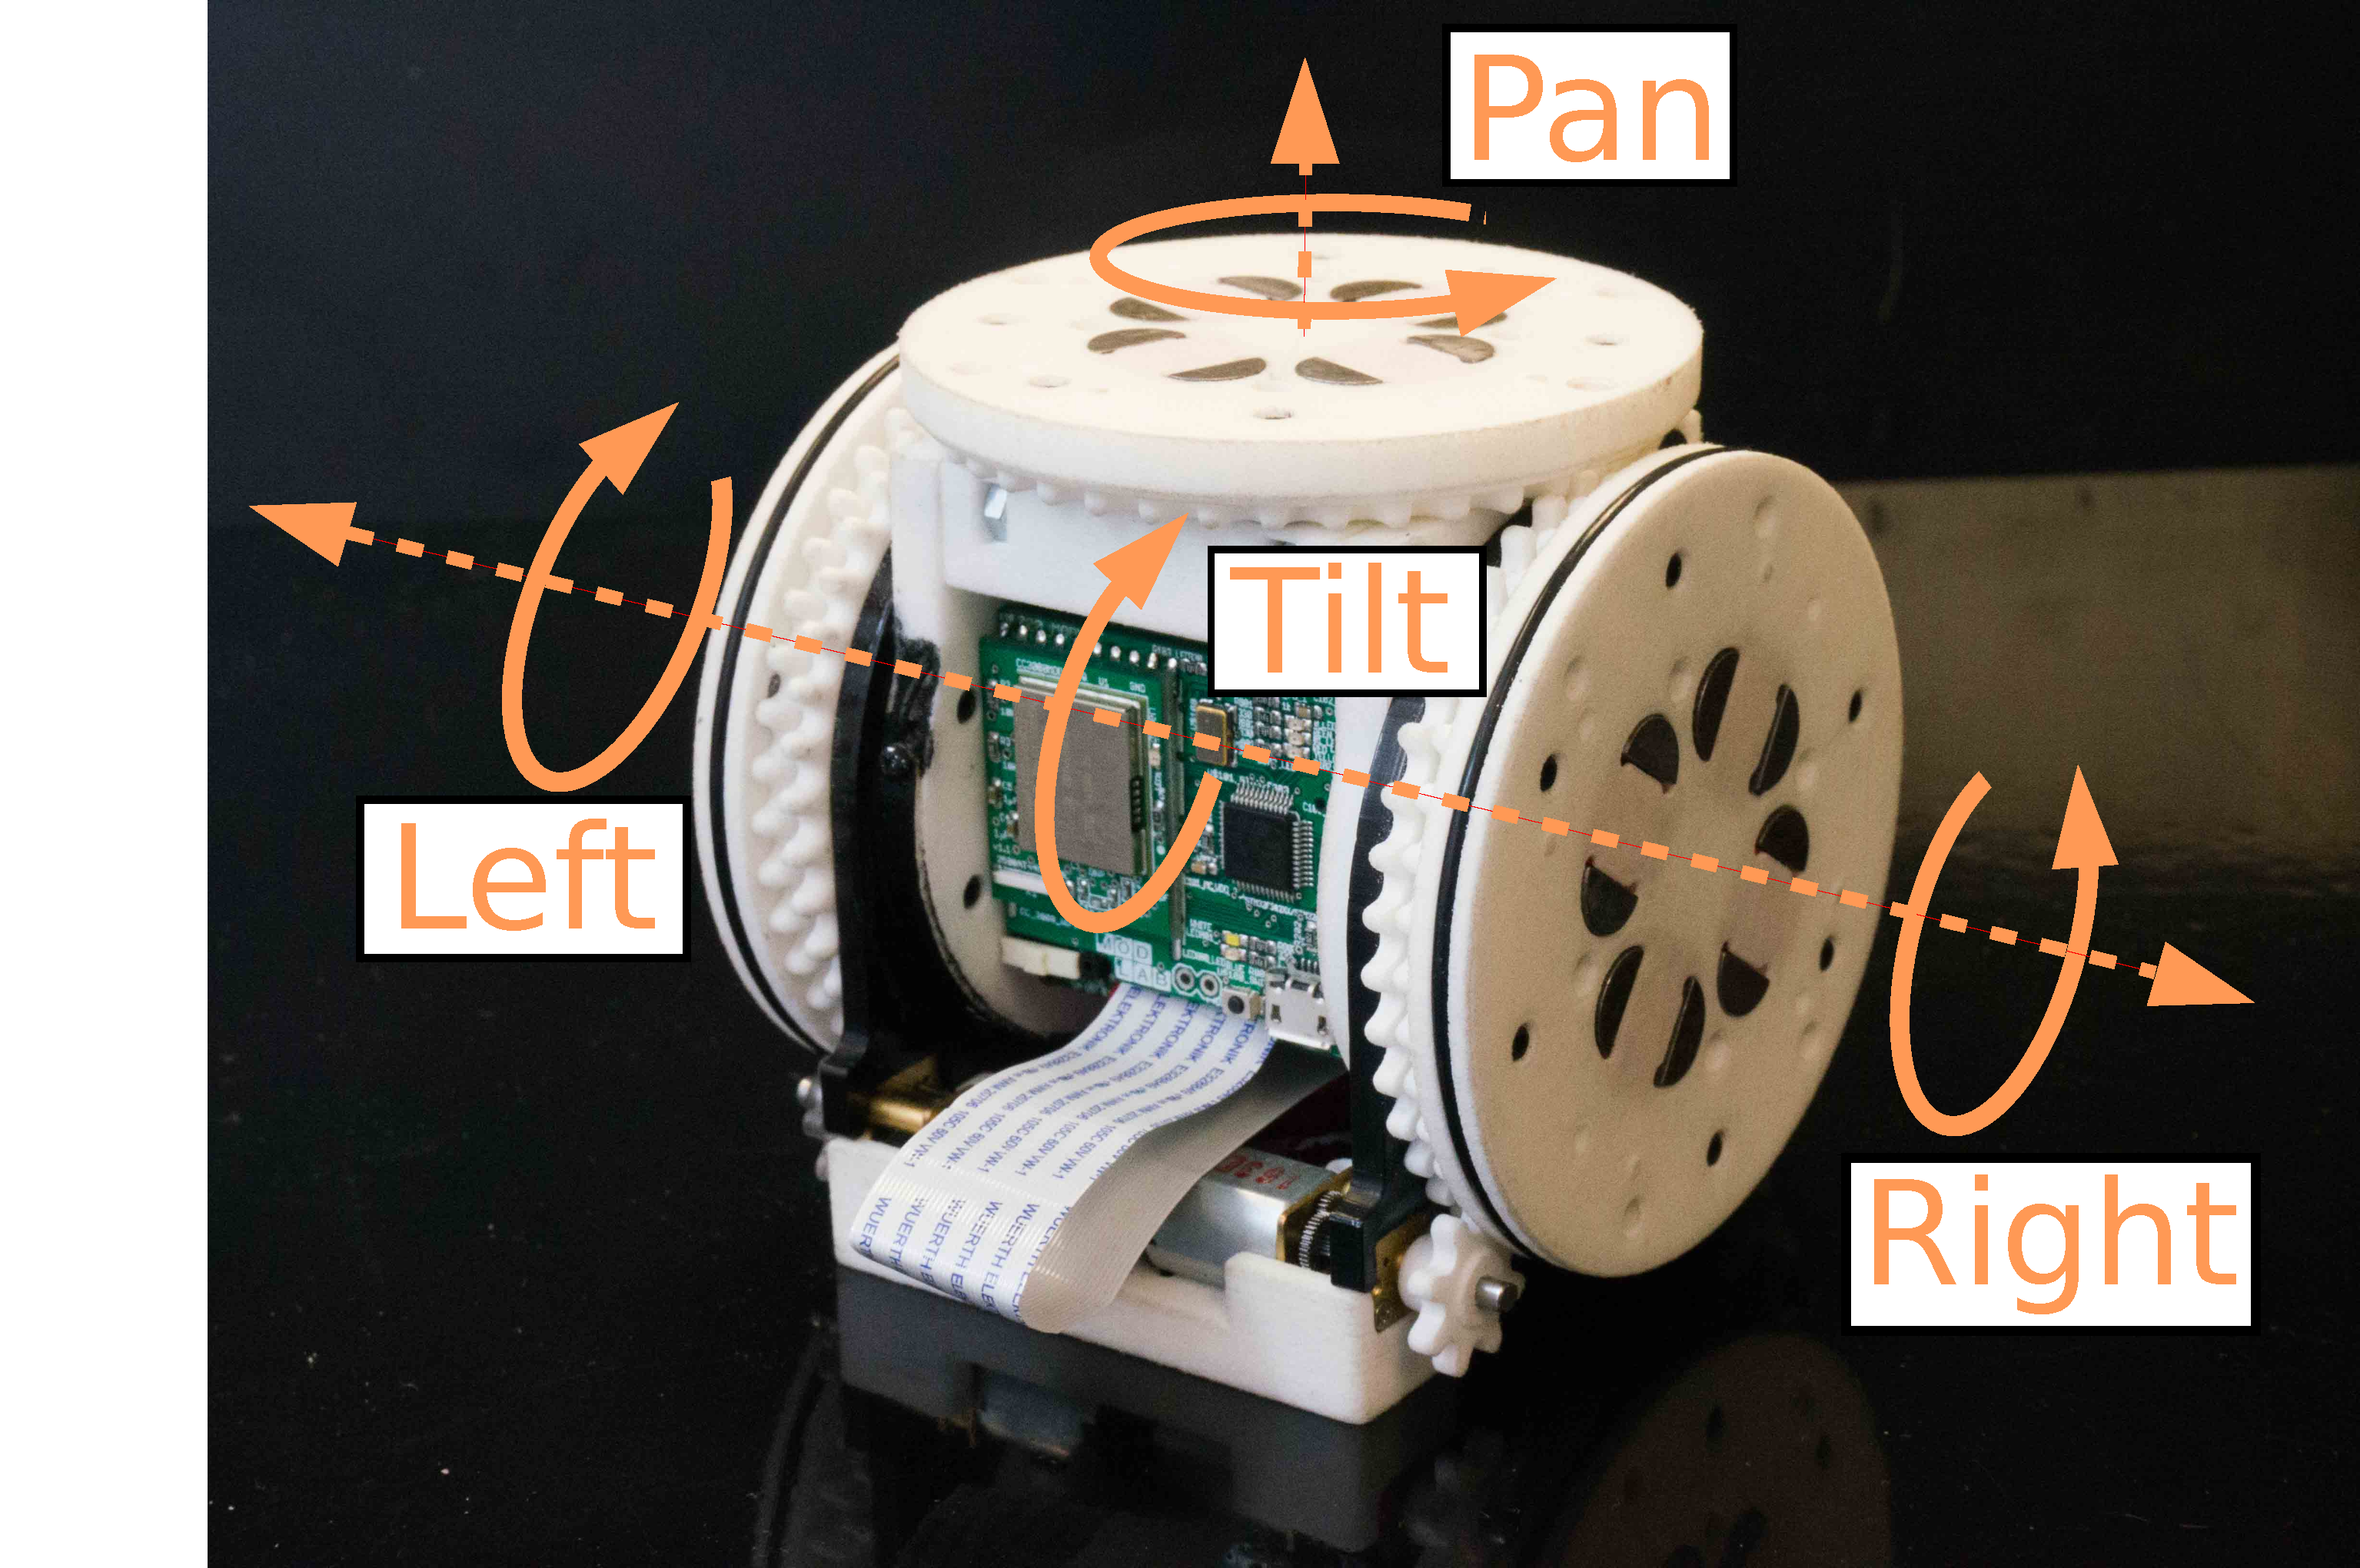
\includegraphics[height=1.5in]{images/smores_dof.pdf}
\end{center}
\caption{SMORES-EP module}
\label{fig:smores-module}
\end{figure}
%

%
\section*{Acknowledgments}
%
This work was funded by NSF grant numbers CNS-1329620 and CNS-1329692.
\TODO{Is this all of them?}


%%%%%%%%%%%%%%%%%%%%%%%%%%%%%%%%%%%%%%%%%%%%%%%%%%%%%%%%%%%%%%%%
%%%                      Bibliography                        %%%
%%%%%%%%%%%%%%%%%%%%%%%%%%%%%%%%%%%%%%%%%%%%%%%%%%%%%%%%%%%%%%%%

%% Use plainnat to work nicely with natbib. 

\bibliographystyle{plainnat}
\bibliography{references}

\end{document}









